\documentclass[9pt,twoside,lineno]{pnas-new}
% Use the lineno option to display guide line numbers if required.

\templatetype{pnassupportinginfo}

\title{Your main manuscript title}
\author{Author1, Author2 and Author3 (complete author list)}
\correspondingauthor{Corresponding Author name.\\E-mail: author.two@email.com}

\begin{document}

%% Comment out or remove this line before generating final copy for submission; this will also remove the warning re: "Consecutive odd pages found".
\instructionspage  

\maketitle

%% Adds the main heading for the SI text. Comment out this line if you do not have any supporting information text.
\SItext


% \subsection*{Subhead}
% Type or paste text here. This should be additional explanatory text such as an extended technical description of results, full details of mathematical models, etc.   
\subsection{Validation}
Samples from cases who report they were exposed abroad can help validate the transmission chains inferred from the phylodynamic tree. Taking reported exposures as the ground truth, we expect cases exposed abroad to be the index cases in Swiss transmission chains. Therefore, we ran a validation analysis taking 

In Switzerland, patient exposure information is recorded in the meldungen zum klinischen befund (MKB)form submitted to the Federal Office for Public Health (FOPH). MKB reporting criteria changed several times during the study period. Beginning 31. January 2020, all symptomatic patients or patients with close exposure to another case were tested, and all positive patients were MKB-reportable. Beginning 13. March 2020, only symptomatic patients with symptoms sufficient for hospitalization, in a risk group, or working in healthcare were tested, and all positive patients were MKB-reportable. Beginning 20. March 2020, only hospitalized patients were MKB-reportable. Beginning 16. April 2020, patients in care homes were also MKB-reportable. Beginning 22. April 2020, all symptomatic patients were tested but the MKB-reporting criteria did not change. Beginning 11. May 2020, all positive patients were again MKB-reportable. Beginning 28. October 2020, again only hospitalized patients or patients in care homes were MKB-reportable. Sources: personal email "Potential exposure data not in the meldeformular?", \url{https://www.covid19healthsystem.org/countries/switzerland/livinghit.aspx?Section=1.5%20Testing&Type=Section}

T

\section*{Heading}
\subsection*{Subhead}
Type or paste text here. You may break this section up into subheads as needed (e.g., one section on ``Materials'' and one on ``Methods'').

\subsection*{Materials}
Add a materials subsection if you need to.

\subsection*{Methods}
Add a methods subsection if you need to.


%%% Each figure should be on its own page
\begin{figure}
\centering
\includegraphics[width=\textwidth]{example-image}
\caption{First figure}
\end{figure}

\begin{figure}
\centering
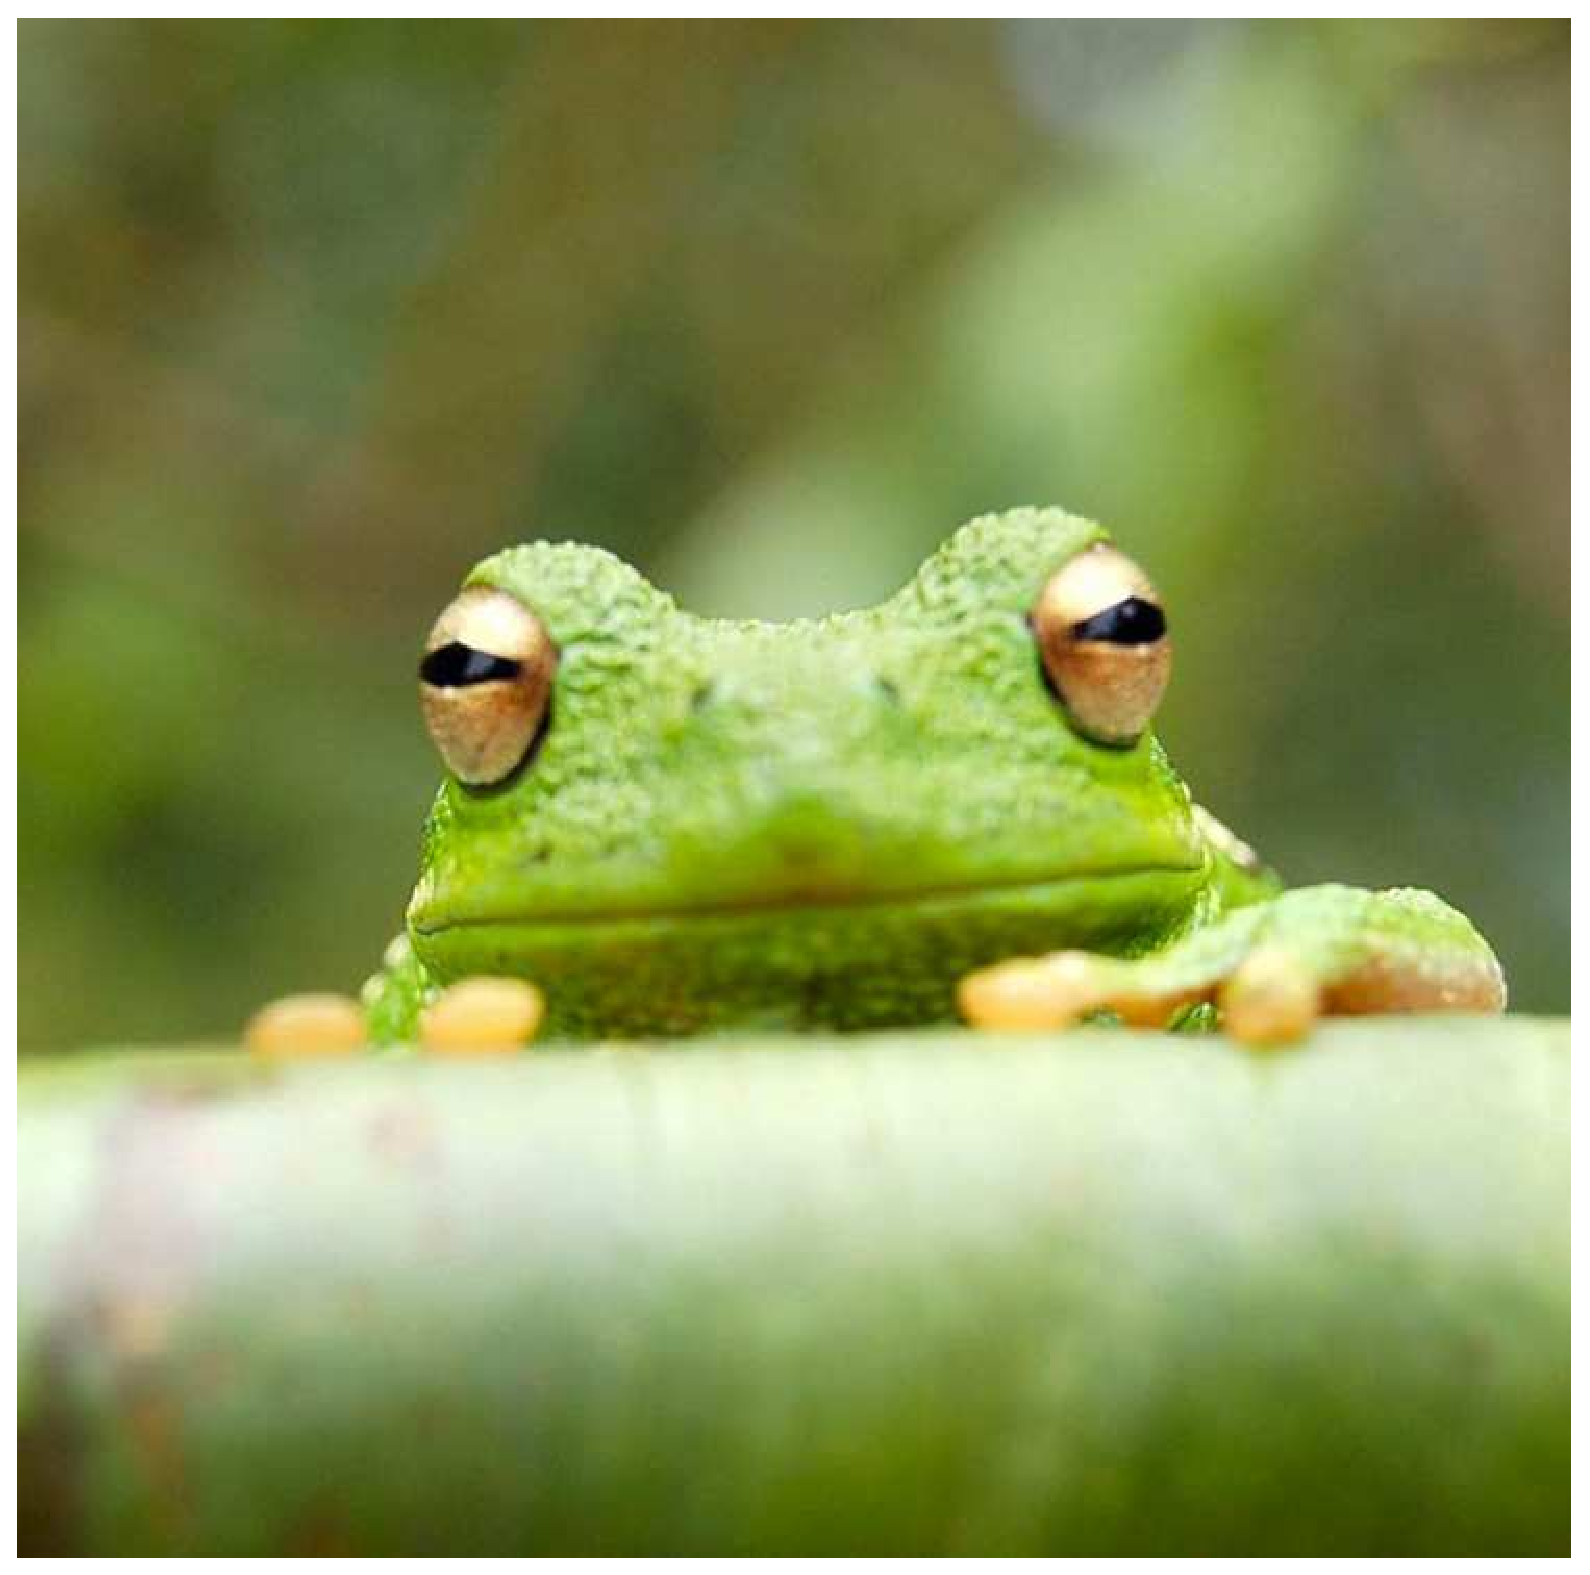
\includegraphics[width=\textwidth]{frog}
\caption{Second figure}
\end{figure}

\begin{table}\centering
\caption{This is a table}

\begin{tabular}{lrrr}
Species & CBS & CV & G3 \\
\midrule
1. Acetaldehyde & 0.0 & 0.0 & 0.0 \\
2. Vinyl alcohol & 9.1 & 9.6 & 13.5 \\
3. Hydroxyethylidene & 50.8 & 51.2 & 54.0\\
\bottomrule
\end{tabular}
\end{table}

%%% Add this line AFTER all your figures and tables
\FloatBarrier

\movie{Type legend for the movie here.}

\movie{Type legend for the other movie here. Adding longer text to show what happens, to decide on alignment and/or indentations.}

\movie{A third movie, just for kicks.}

\dataset{dataset_one.txt}{Type or paste legend here.}

\dataset{dataset_two.txt}{Type or paste legend here. Adding longer text to show what happens, to decide on alignment and/or indentations for multi-line or paragraph captions.}

\bibliography{pnas-sample}

\end{document}
